% **************************************************************************************************************
% A Classic Thesis Style
% An Homage to The Elements of Typographic Style
%
% Copyright (C) 2018 André Miede and Ivo Pletikosić
%
% If you like the style then I would appreciate a postcard. My address
% can be found in the file ClassicThesis.pdf. A collection of the
% postcards I received so far is available online at
% http://postcards.miede.de
%
% License:
% This program is free software; you can redistribute it and/or modify
% it under the terms of the GNU General Public License as published by
% the Free Software Foundation; either version 2 of the License, or
% (at your option) any later version.
%
% This program is distributed in the hope that it will be useful,
% but WITHOUT ANY WARRANTY; without even the implied warranty of
% MERCHANTABILITY or FITNESS FOR A PARTICULAR PURPOSE.  See the
% GNU General Public License for more details.
%
% You should have received a copy of the GNU General Public License
% along with this program; see the file COPYING.  If not, write to
% the Free Software Foundation, Inc., 59 Temple Place - Suite 330,
% Boston, MA 02111-1307, USA.
%
% PLEASE SEE ALSO THE AUTHORS' NOTE REGARDING THIS LICENSE
% IN THE DOCUMENTATION (ClassicThesis.pdf --> Chapter 1 / Chapter01.tex)
% **************************************************************************************************************
\RequirePackage{silence} % :-\
    \WarningFilter{scrreprt}{Usage of package `titlesec'}
    %\WarningFilter{scrreprt}{Activating an ugly workaround}
    \WarningFilter{titlesec}{Non standard sectioning command detected}
\documentclass[ twoside,openright,titlepage,numbers=noenddot,%1headlines,
                headinclude,footinclude,cleardoublepage=empty,abstract=on,
                BCOR=5mm,paper=a4,fontsize=11pt
                ]{scrreprt}

%********************************************************************
% Note: Make all your adjustments in here
%*******************************************************
%%%%%%%%%%%%%%%%%%%%%%%%%%%%%%%%%%%%%%%%%
% Classicthesis Typographic Thesis
% Configuration File
%
% This file has been downloaded from:
% http://www.LaTeXTemplates.com
%
% Original author:
% André Miede (http://www.miede.de) with extensive commenting changes by:
% Vel (vel@LaTeXTemplates.com)
%
% License:
% GNU General Public License (v2)
%
% Important note:
% The main lines to change in this file are in the DOCUMENT VARIABLES
% section, the rest of the file is for advanced configuration.
%
%%%%%%%%%%%%%%%%%%%%%%%%%%%%%%%%%%%%%%%%%

%----------------------------------------------------------------------------------------
%	CHARACTER ENCODING
%----------------------------------------------------------------------------------------

\PassOptionsToPackage{utf8}{inputenc} % Set the encoding of your files. UTF-8 is the only sensible encoding nowadays. If you can't read äöüßáéçèê∂åëæƒÏ€ then change the encoding setting in your editor, not the line below. If your editor does not support utf8 use another editor!
\usepackage{inputenc}

%----------------------------------------------------------------------------------------
%	DOCUMENT VARIABLES
%	Fill in the lines below to enter your information into the thesis template
%	Each of the commands can be cited anywhere in the thesis
%----------------------------------------------------------------------------------------

% Remove drafting to get rid of the '[ Date - classicthesis version 4.0 ]' text at the bottom of every page
\PassOptionsToPackage{eulerchapternumbers,listings,drafting, pdfspacing, subfig,beramono,eulermath,parts}{classicthesis}
% Available options: drafting parts nochapters linedheaders eulerchapternumbers beramono eulermath pdfspacing minionprospacing tocaligned dottedtoc manychapters listings floatperchapter subfig

\newcommand{\myTitle}{Calculus I\xspace}
\newcommand{\mySubtitle}{Fuck yeah\xspace}
\newcommand{\myDegree}{Magnifico\xspace}
\newcommand{\myName}{Riccardo Cereghino\xspace}
\newcommand{\myProf}{Ernesto De Vito\xspace}
\newcommand{\myOtherProf}{Put name here\xspace}
\newcommand{\mySupervisor}{Put name here\xspace}
\newcommand{\myFaculty}{Informatica\xspace}
\newcommand{\myDepartment}{DIBRIS\xspace}
\newcommand{\myUni}{Put data here\xspace}
\newcommand{\myLocation}{Rapallo\xspace}
\newcommand{\myTime}{Febbraio 2019\xspace}
\newcommand{\myVersion}{version 4.2\xspace}

%----------------------------------------------------------------------------------------
%	USEFUL COMMANDS
%----------------------------------------------------------------------------------------

\newcommand{\ie}{i.\,e.}
\newcommand{\Ie}{I.\,e.}
\newcommand{\eg}{e.\,g.}
\newcommand{\Eg}{E.\,g.} 

\newcounter{dummy} % Necessary for correct hyperlinks (to index, bib, etc.)
\providecommand{\mLyX}{L\kern-.1667em\lower.25em\hbox{Y}\kern-.125emX\@}
\newlength{\abcd} % for ab..z string length calculation

%----------------------------------------------------------------------------------------
%	PACKAGES
%----------------------------------------------------------------------------------------

\usepackage{lipsum} % Used for inserting dummy 'Lorem ipsum' text into the template

%------------------------------------------------

%\PassOptionsToPackage{ngerman,american}{babel}  % Change this to your language(s)
% Spanish languages need extra options in order to work with this template
%\PassOptionsToPackage{spanish,es-lcroman}{babel}
\usepackage{babel}

%------------------------------------------------			

\usepackage{csquotes}
\PassOptionsToPackage{%
%backend=biber, % Instead of bibtex
backend=bibtex8,bibencoding=ascii,%
language=auto,%
style=numeric-comp,%
%style=authoryear-comp, % Author 1999, 2010
%bibstyle=authoryear,dashed=false, % dashed: substitute rep. author with ---
sorting=nyt, % name, year, title
maxbibnames=10, % default: 3, et al.
%backref=true,%
natbib=true % natbib compatibility mode (\citep and \citet still work)
}{biblatex}
\usepackage{biblatex}
 
 %------------------------------------------------

\PassOptionsToPackage{fleqn}{amsmath} % Math environments and more by the AMS 
 \usepackage{amsmath}
 
 %------------------------------------------------

\PassOptionsToPackage{T1}{fontenc} % T2A for cyrillics
\usepackage{fontenc}

%------------------------------------------------

\usepackage{textcomp} % Fix warning with missing font shapes

%------------------------------------------------

\usepackage{scrhack} % Fix warnings when using KOMA with listings package  

%------------------------------------------------

\usepackage{xspace} % To get the spacing after macros right

%------------------------------------------------

\usepackage{mparhack} % To get marginpar right

%------------------------------------------------

%\usepackage{fixltx2e} % Fixes some LaTeX stuff 

%------------------------------------------------

\PassOptionsToPackage{smaller}{acronym} % Include printonlyused in the first bracket to only show acronyms used in the text
\usepackage{acronym} % Nice macros for handling all acronyms in the thesis

%\renewcommand*{\acsfont}[1]{\textssc{#1}} % For MinionPro
\renewcommand*{\aclabelfont}[1]{\acsfont{#1}}

%------------------------------------------------

\PassOptionsToPackage{pdftex}{graphicx}
\usepackage{graphicx} 

%----------------------------------------------------------------------------------------
%	FLOATS: TABLES, FIGURES AND CAPTIONS SETUP
%----------------------------------------------------------------------------------------

\usepackage{tabularx} % Better tables
\setlength{\extrarowheight}{3pt} % Increase table row height
\newcommand{\tableheadline}[1]{\multicolumn{1}{c}{\spacedlowsmallcaps{#1}}}
\newcommand{\myfloatalign}{\centering} % To be used with each float for alignment
\usepackage{caption}
\captionsetup{font=small}
\usepackage{subfig}  

%----------------------------------------------------------------------------------------
%	CODE LISTINGS SETUP
%----------------------------------------------------------------------------------------

\usepackage{listings} 
%\lstset{emph={trueIndex,root},emphstyle=\color{BlueViolet}}%\underbar} % For special keywords
\lstset{language=[LaTeX]Tex,%C++ % Specify the language(s) for listings here
morekeywords={PassOptionsToPackage,selectlanguage},
keywordstyle=\color{RoyalBlue}, % Add \bfseries for bold
basicstyle=\small\ttfamily, % Makes listings a smaller font size and a different font
%identifierstyle=\color{NavyBlue}, % Color of text inside brackets
commentstyle=\color{Green}\ttfamily, % Color of comments
stringstyle=\rmfamily, % Font type to use for strings
numbers=left, % Change left to none to remove line numbers
numberstyle=\scriptsize, % Font size of the line numbers
stepnumber=5, % Increment of line numbers
numbersep=8pt, % Distance of line numbers from code listing
showstringspaces=false, % Sets whether spaces in strings should appear underlined
breaklines=true, % Force the code to stay in the confines of the listing box
%frameround=ftff, % Uncomment for rounded frame
%frame=single, % Frame border - none/leftline/topline/bottomline/lines/single/shadowbox/L
belowcaptionskip=.75\baselineskip % Space after the "Listing #: Desciption" text and the listing box
}

%----------------------------------------------------------------------------------------
%	HYPERREFERENCES
%----------------------------------------------------------------------------------------

\PassOptionsToPackage{pdftex,hyperfootnotes=false,pdfpagelabels}{hyperref}
\usepackage{hyperref}  % backref linktocpage pagebackref
\pdfcompresslevel=9
\pdfadjustspacing=1

\hypersetup{
% Uncomment the line below to remove all links (to references, figures, tables, etc), useful for b/w printouts
%draft, 
colorlinks=true, linktocpage=true, pdfstartpage=3, pdfstartview=FitV,
% Uncomment the line below if you want to have black links (e.g. for printing black and white)
%colorlinks=false, linktocpage=false, pdfborder={0 0 0}, pdfstartpage=3, pdfstartview=FitV, 
breaklinks=true, pdfpagemode=UseNone, pageanchor=true, pdfpagemode=UseOutlines,%
plainpages=false, bookmarksnumbered, bookmarksopen=true, bookmarksopenlevel=1,%
hypertexnames=true, pdfhighlight=/O,%nesting=true,%frenchlinks,%
urlcolor=webbrown, linkcolor=RoyalBlue, citecolor=webgreen, %pagecolor=RoyalBlue,%
    %urlcolor=Black, linkcolor=Black, citecolor=Black, %pagecolor=Black,%
%------------------------------------------------
% PDF file meta-information
pdftitle={\myTitle},
pdfauthor={\textcopyright\ \myName, \myUni, \myFaculty},
pdfsubject={},
pdfkeywords={},
pdfcreator={pdfLaTeX},
pdfproducer={LaTeX with hyperref and classicthesis}
%------------------------------------------------
}

%----------------------------------------------------------------------------------------
%	AUTOREFERENCES SETUP
%	Redefines how references in text are prefaced for different 
%	languages (e.g. "Section 1.2" or "section 1.2")
%----------------------------------------------------------------------------------------

\makeatletter
\@ifpackageloaded{babel}
{
\addto\extrasamerican{
\renewcommand*{\figureautorefname}{Figure}
\renewcommand*{\tableautorefname}{Table}
\renewcommand*{\partautorefname}{Part}
\renewcommand*{\chapterautorefname}{Chapter}
\renewcommand*{\sectionautorefname}{Section}
\renewcommand*{\subsectionautorefname}{Section}
\renewcommand*{\subsubsectionautorefname}{Section}
}
\addto\extrasngerman{
\renewcommand*{\paragraphautorefname}{Absatz}
\renewcommand*{\subparagraphautorefname}{Unterabsatz}
\renewcommand*{\footnoteautorefname}{Fu\"snote}
\renewcommand*{\FancyVerbLineautorefname}{Zeile}
\renewcommand*{\theoremautorefname}{Theorem}
\renewcommand*{\appendixautorefname}{Anhang}
\renewcommand*{\equationautorefname}{Gleichung}
\renewcommand*{\itemautorefname}{Punkt}
}
\providecommand{\subfigureautorefname}{\figureautorefname} % Fix to getting autorefs for subfigures right
}{\relax}
\makeatother

\usepackage{amssymb}

\let\numberset\mathbb
\newcommand{\N}{\numberset{N}}
\newcommand{\Z}{\numberset{Z}}
\newcommand{\Q}{\numberset{Q}}
\newcommand{\R}{\numberset{R}}
\newcommand{\C}{\numberset{C}}
\newcommand{\U}{\numberset{U}}
\newcommand{\I}{\numberset{I}}
\newcommand{\PP}{\numberset{P}}
\newcommand{\CC}{\complement}
\newcommand{\dom}{\text{dom }}
\newcommand{\im}{\text{Im }}
\usepackage{float}
\usepackage{wrapfig}
%----------------------------------------------------------------------------------------

\usepackage{classicthesis} 

%----------------------------------------------------------------------------------------
%	CHANGING TEXT AREA 
%----------------------------------------------------------------------------------------

%\linespread{1.05} % a bit more for Palatino
%\areaset[current]{312pt}{761pt} % 686 (factor 2.2) + 33 head + 42 head \the\footskip
%\setlength{\marginparwidth}{7em}%
%\setlength{\marginparsep}{2em}%

%----------------------------------------------------------------------------------------
%	USING DIFFERENT FONTS
%----------------------------------------------------------------------------------------

%\usepackage[oldstylenums]{kpfonts} % oldstyle notextcomp
%\usepackage[osf]{libertine}
%\usepackage[light,condensed,math]{iwona}
%\renewcommand{\sfdefault}{iwona}
%\usepackage{lmodern} % <-- no osf support :-(
%\usepackage{cfr-lm} % 
%\usepackage[urw-garamond]{mathdesign} <-- no osf support :-(
%\usepackage[default,osfigures]{opensans} % scale=0.95 
%\usepackage[sfdefault]{FiraSans}


\theoremstyle{break}
\newtheorem{teo}{Teorema}[chapter]
\newtheorem{prop}{Proposizione}[chapter]
%********************************************************************
% Bibliographies
%*******************************************************
%\addbibresource{Bibliography.bib}
%\addbibresource[label=ownpubs]{AMiede_Publications.bib}

%********************************************************************
% Hyphenation
%*******************************************************
%\hyphenation{put special hyphenation here}

% ********************************************************************
% GO!GO!GO! MOVE IT!
%*******************************************************
\begin{document}
\frenchspacing
\raggedbottom
\selectlanguage{italian} % american ngerman
%\renewcommand*{\bibname}{new name}
%\setbibpreamble{}
\pagenumbering{roman}
\pagestyle{plain}
%********************************************************************
% Frontmatter
%*******************************************************
%%*******************************************************
% Little Dirty Titlepage
%*******************************************************
\thispagestyle{empty}
%\pdfbookmark[1]{Titel}{title}
%*******************************************************
\begin{center}
    \spacedlowsmallcaps{\myName} \\ \medskip

    \begingroup
        \color{CTtitle}\spacedallcaps{\myTitle}
    \endgroup
\end{center}

%*******************************************************
% Titlepage
%*******************************************************
\begin{titlepage}
    %\pdfbookmark[1]{\myTitle}{titlepage}
    % if you want the titlepage to be centered, uncomment and fine-tune the line below (KOMA classes environment)
    \begin{addmargin}[-1cm]{-3cm}
    \begin{center}
        \large

        \hfill

        \vfill

        \begingroup
            \color{CTtitle}\spacedallcaps{\myTitle} \\ \bigskip
        \endgroup

        \spacedlowsmallcaps{\myName}

        \vfill

        
\includegraphics[width=6cm]{gfx/brand.jpg} \\ \medskip

        \mySubtitle \\ \medskip
        %\myDegree \\
        \myDepartment \\
        \myFaculty \\
        \myUni \\ \bigskip

        %\myTime

        \vfill

    \end{center}
  \end{addmargin}
\end{titlepage}

%\thispagestyle{empty}

\hfill

\vfill

\noindent\myName: \textit{\myTitle,} \mySubtitle, %\myDegree,
\textcopyright\ \myTime

%\bigskip
%
%\noindent\spacedlowsmallcaps{Supervisors}: \\
%\myProf \\
%\myOtherProf \\
%\mySupervisor
%
%\medskip
%
%\noindent\spacedlowsmallcaps{Location}: \\
%\myLocation
%
%\medskip
%
%\noindent\spacedlowsmallcaps{Time Frame}: \\
%\myTime

%\cleardoublepage%*******************************************************
% Dedication
%*******************************************************
\thispagestyle{empty}
\phantomsection
\pdfbookmark[1]{Dedication}{Dedication}

\vspace*{3cm}

\begin{center}
    \emph{Ohana} means family. \\
    Family means nobody gets left behind, or forgotten. \\ \medskip
    --- Lilo \& Stitch
\end{center}

\medskip

\begin{center}
    Dedicated to the loving memory of Rudolf Miede. \\ \smallskip
    1939\,--\,2005
\end{center}

%\cleardoublepage\include{FrontBackmatter/Foreword}
%\cleardoublepage%*******************************************************
% Abstract
%*******************************************************
%\renewcommand{\abstractname}{Abstract}
\pdfbookmark[1]{Abstract}{Abstract}
% \addcontentsline{toc}{chapter}{\tocEntry{Abstract}}
\begingroup
\let\clearpage\relax
\let\cleardoublepage\relax
\let\cleardoublepage\relax

\chapter*{Abstract}
Short summary of the contents in English\dots a great guide by
Kent Beck how to write good abstracts can be found here:
\begin{center}
\url{https://plg.uwaterloo.ca/~migod/research/beckOOPSLA.html}
\end{center}

\vfill

\begin{otherlanguage}{ngerman}
\pdfbookmark[1]{Zusammenfassung}{Zusammenfassung}
\chapter*{Zusammenfassung}
Kurze Zusammenfassung des Inhaltes in deutscher Sprache\dots
\end{otherlanguage}

\endgroup

\vfill

%\cleardoublepage%*******************************************************
% Publications
%*******************************************************
\pdfbookmark[1]{Publications}{publications}
\chapter*{Publications}\graffito{This is just an early --~and currently ugly~-- test!}
This might come in handy for PhD theses: some ideas and figures have appeared previously in the following publications:

%\noindent Put your publications from the thesis here. The packages \texttt{multibib} or \texttt{bibtopic} etc. can be used to handle multiple different bibliographies in your document.

\begin{refsection}[ownpubs]
    \small
    \nocite{*} % is local to to the enclosing refsection
    \printbibliography[heading=none]
\end{refsection}

\emph{Attention}: This requires a separate run of \texttt{bibtex} for your \texttt{refsection}, \eg, \texttt{ClassicThesis1-blx} for this file. You might also use \texttt{biber} as the backend for \texttt{biblatex}. See also \url{http://tex.stackexchange.com/questions/128196/problem-with-refsection}.

%\cleardoublepage%*******************************************************
% Acknowledgments
%*******************************************************
\pdfbookmark[1]{Acknowledgments}{acknowledgments}

\begin{flushright}{\slshape
    We have seen that computer programming is an art, \\
    because it applies accumulated knowledge to the world, \\
    because it requires skill and ingenuity, and especially \\
    because it produces objects of beauty.} \\ \medskip
    --- \defcitealias{knuth:1974}{Donald E. Knuth}\citetalias{knuth:1974} \citep{knuth:1974}
\end{flushright}



\bigskip

\begingroup
\let\clearpage\relax
\let\cleardoublepage\relax
\let\cleardoublepage\relax
\chapter*{Acknowledgments}
Put your acknowledgments here.

Many thanks to everybody who already sent me a postcard!

Regarding the typography and other help, many thanks go to Marco
Kuhlmann, Philipp Lehman, Lothar Schlesier, Jim Young, Lorenzo
Pantieri and Enrico Gregorio\footnote{Members of GuIT (Gruppo
Italiano Utilizzatori di \TeX\ e \LaTeX )}, J\"org Sommer,
Joachim K\"ostler, Daniel Gottschlag, Denis Aydin, Paride
Legovini, Steffen Prochnow, Nicolas Repp, Hinrich Harms,
Roland Winkler, Jörg Weber, Henri Menke, Claus Lahiri,
Clemens Niederberger, Stefano Bragaglia, Jörn Hees,
Scott Lowe, Dave Howcroft, Jos\'e M. Alcaide, David Carlisle,
Ulrike Fischer, Hugues de Lassus, Csaba Hajdu, Dave Howcroft, 
and the whole \LaTeX-community for support, ideas and
some great software.

\bigskip

\noindent\emph{Regarding \mLyX}: The \mLyX\ port was intially done by
\emph{Nicholas Mariette} in March 2009 and continued by
\emph{Ivo Pletikosi\'c} in 2011. Thank you very much for your
work and for the contributions to the original style.


\endgroup

\cleardoublepage%*******************************************************
% Table of Contents
%*******************************************************
\pagestyle{scrheadings}
%\phantomsection
\pdfbookmark[1]{\contentsname}{tableofcontents}
\setcounter{tocdepth}{2} % <-- 2 includes up to subsections in the ToC
\setcounter{secnumdepth}{3} % <-- 3 numbers up to subsubsections
\manualmark
\markboth{\spacedlowsmallcaps{\contentsname}}{\spacedlowsmallcaps{\contentsname}}
\tableofcontents
\automark[section]{chapter}
\renewcommand{\chaptermark}[1]{\markboth{\spacedlowsmallcaps{#1}}{\spacedlowsmallcaps{#1}}}
\renewcommand{\sectionmark}[1]{\markright{\textsc{\thesection}\enspace\spacedlowsmallcaps{#1}}}
%*******************************************************
% List of Figures and of the Tables
%*******************************************************
\clearpage
% \pagestyle{empty} % Uncomment this line if your lists should not have any headlines with section name and page number
\begingroup
    \let\clearpage\relax
    \let\cleardoublepage\relax
    %*******************************************************
    % List of Figures
    %*******************************************************
    %\phantomsection
    %\addcontentsline{toc}{chapter}{\listfigurename}
    \pdfbookmark[1]{\listfigurename}{lof}
    \listoffigures

    \vspace{8ex}

    %*******************************************************
    % List of Tables
    %*******************************************************
    %\phantomsection
    %\addcontentsline{toc}{chapter}{\listtablename}
    \pdfbookmark[1]{\listtablename}{lot}
    \listoftables

    \vspace{8ex}
    % \newpage

    %*******************************************************
    % List of Listings
    %*******************************************************
    %\phantomsection
    %\addcontentsline{toc}{chapter}{\lstlistlistingname}
    \pdfbookmark[1]{\lstlistlistingname}{lol}
    \lstlistoflistings

    \vspace{8ex}

    %*******************************************************
    % Acronyms
    %*******************************************************
    %\phantomsection
    \pdfbookmark[1]{Acronyms}{acronyms}
    \markboth{\spacedlowsmallcaps{Acronyms}}{\spacedlowsmallcaps{Acronyms}}
    \chapter*{Acronyms}
    \begin{acronym}[UMLX]
        \acro{DRY}{Don't Repeat Yourself}
        \acro{API}{Application Programming Interface}
        \acro{UML}{Unified Modeling Language}
    \end{acronym}

\endgroup

%********************************************************************
% Mainmatter
%*******************************************************
\cleardoublepage
\pagestyle{scrheadings}
\pagenumbering{arabic}
%\setcounter{page}{90}
% use \cleardoublepage here to avoid problems with pdfbookmark
\cleardoublepage
\part{Introduzione}\label{pt:intro}
% Chapter 1

\chapter{Notazione} % Chapter title

\label{ch:notazione} % For referencing the chapter elsewhere, use \autoref{ch:introduction} 

%----------------------------------------------------------------------------------------
Un richiamo alla notazione che verrà utilizzata nel documento.

\section{Insiemistica}
\begin{tabular}{|l|l|}
  \hline
  $\emptyset$ & Insieme vuoto \\
  $\N$ & Insieme dei numeri naturali compreso lo $0$ \\
  $\Z$ & Insieme dei numeri relativi \\
  $\Q$ & Insieme dei numeri razionali \\
  $\R$ & Insieme dei numeri reali \\\hline
\end{tabular}

\section{Simboli logici}
\begin{tabular}{|l|l|}
  \hline
  $| $ & tale che \\
  $ \Rightarrow $ & implica \\
  $ \Leftrightarrow $ & se e solo se \\
  $ \forall $ & per ogni \\
  $ \exists $ & esiste \\
  $ \nexists $ & non esiste \\
  $ \in $ & appartiene \\
  $ \notin $ & non appartiene \\\hline
\end{tabular}



\subsection{Intervalli}
\begin{tabular}{|l|l|}
\hline
intervallo limitato chiuso &$[a,b] = \left\{ x\in \R \middle| a \leq x \leq b \right\}$ \\
intervallo limitato aperto&$(a,b) = \left\{ x\in \R \middle| a < x < b \right\}$ \\
intervallo limitato aperto a destra&$[a,b) = \left\{ x\in \R \middle| a \leq x < b \right\}$ \\
intervallo limitato aperto a sinistra&$(a,b] = \left\{ x\in \R \middle| a < x \leq b \right\}$ \\
intervallo illimitato chiuso a sinistra&$[a,+\infty) = \left\{ x\in \R \middle| x \geq a \right\}$ \\
intervallo illimitato aperto a sinistra&$(a,+\infty) = \left\{ x\in \R \middle| x > a \right\}$ \\
intervallo illimitato chiuso a destra&$(-\infty,b] = \left\{ x\in \R \middle| x \leq b \right\}$ \\
intervallo illimitato aperto a destra&$(-\infty,b) = \left\{ x\in \R \middle| x < b \right\}$ \\
intervallo illimitato&$(-\infty,+\infty) = \R$ \\ \hline
\end{tabular}

\section{Insiemi}
\subsection{Relazioni tra insiemi}
Dati due insiemi $A$ e $B$:

\begin{description}
  \item[Inclusione:] si dice che $A$ è un sottoinsieme di $B$, o che è contenuto in $B$:
    \[A \subseteq  B\]
    \[\forall x \in A \Rightarrow x \in B\]
  \item[Inclusione propria:]
    \[A \subsetneqq  B\]
    \[
      \begin{cases}
        \forall x \in A \Rightarrow x \in B \\
        \exists x \in B | x \notin A
        \end{cases}
      \]
\end{description}

\subsection{Operazioni tra insiemi}
\begin{description}
  \item[Intersezione:]
    \[A \cap B = \left\{ x \in X \middle| x \in A, x \in B\right\}\]
  \item[Unione:]
    \[A \cup B = \left\{ x \in X \middle| x \in A or x \in B\right\}\]
  \item[Differenza insiemistica:]
    \[A \diagdown B = \left\{ x \in X \middle| x \in A, x \notin B\right\}\]
  \item[Complementare:]
    \[A^C = \left\{ x \in X \middle| x \notin A \right\}\]
  \item[Prodotto cartesiano:] dove $(x,y)$ denota la coppia ordinata
  \[A\times B = \left\{ (x,y) \middle| x\in A, y\in B\right\}\]
\end{description}

\section{Numeri reali}
Dati $x,y,z \in \R$ sono definite le operazioni di:
\begin{itemize}
\item somma $x+y$
\item prodotto $xy$
\item relazione d'ordine $x<y$
\end{itemize}
Che soddisfano le seguenti proprietà:

\begin{description}
  \item[Associativa.]
    \[(x+y)+z=x+(y+z)=x+y+z \]
    \[(xy)z=x(yz)=xyz \]
  \item[Commutativa.]
    \[x+y=y+x\]
    \[xy=yx\]
  \item[Distributiva.]
    \[x(y+z)=xy+xz\]
  \item[Esistenza dell'elemento neutro.]
    \[x+0=0+x=x\]
    \[1x=x1=x\]
  \item[Esistenza dell'inverso.]
      \[\forall x \in \R \quad \exists !x=-x \in \R | x+(-x)=0\]
      \[\forall x \in \R \quad x \neq 0 \quad \exists !y=\frac{1}{x} \in \R | x\frac{1}{x}=1 \]
  \item[Relazione d'ordine totale.] per ogni $x,y,z \in \R$ una ed una sola delle seguenti relazioni è vera.
    \[
    \begin{cases}
      x<y \\
      x=y \\
      x>y
    \end{cases}
    \]
  \item[Transitiva.]
    \[(x<y) \cap (y<z) \Rightarrow (x<z)\]
  \item[Compatibilità con la somma.]
    \[x<y \Rightarrow x+z<y+z\]
  \item[Compatibilità con il prodotto.]
    \[x<y \cap z>0 \Rightarrow xz<yz\]
    \[x<y \cap z<0 \Rightarrow xz>yz\]
\end{description}

\section{Geometria}
\subsection{Circonferenza}
Dato il centro di una circonferenza $C=(x_c,y_c)$
Si esprime l'equazione della circonferenza nella forma:
\[(x-x_c)^2+(y-y_c)^2=r^2\]
Oppure:
\[x^2+y^2+\alpha x+ \beta y +\gamma =r^2\]
Per cui se $O=(0,0)$
\[x^2+y^2=r^2\]


\subsubsection{Forma canonica:}
\[\alpha = -2x_c \quad \beta = -2y_c \quad \gamma = x_c^2 + y_c^2 - r^2\]
\[x^2+y^2+\alpha x+ \beta y +\gamma =r^2\]

Per ricavare il centro:
\[C=\left(-\frac{\alpha}{2}, -\frac{\beta}{2}\right)\]
Per ricavare il raggio:
\[r=\sqrt{\frac{\alpha^2}{4}+\frac{\beta^2}{4}-\gamma}\]

\section{Ellisse}
Equazione dell'ellisse (con centro nell'origine degli assi)
\[\frac{x^2}{a^2}+\frac{y^2}{b^2} \qquad a\neq 0 , b\neq 0\]

\cleardoublepage
%\ctparttext{}
\part{Funzioni}\label{pt:funzioni}
% Chapter 2

\chapter{Funzioni elementari di variabile reale} % Chapter title

\label{ch:funzioni-elementari} % For referencing the chapter elsewhere, use \autoref{ch:introduction} 

%----------------------------------------------------------------------------------------

\section{Il concetto di funzione}
\textbf{Definizione:} una funzione $f: A \rightarrow \R$ dove $A \subseteq \R$ è una legge che assegna ad ogni $x\in A$ uno ed un solo valore $y=f(x) \in \R$

\textit{Nota:} in questo caso, i valori di $A$ sono chiamati variabile indipendente $(x)$, mentre  $\R$ è la variabile dipendente $y=f(x)$

\textit{Nota:} inoltre definiamo $A=dom \quad f$ come il dominio della funzione.

\textbf{Definizione:} Il grafico di $f$:
	\[f=\left\{ (x,y) \in \R^2 \middle| x \in A, y=f(x) \right\}\]

\textbf{Definizione:} L'immagine di $f$, Im f:
	\[f(A)=\left\{ f(x) \in \R \middle| x \in A \right\}\]

\section{Operazioni tra funzioni}
Date due funzioni $f:A\rightarrow \R \qquad g:B\rightarrow \R$
\begin{description}
	\item[Somma e differenza:] $(f+g)(x)=f(x)+g(x) \qquad dom(f+g)=A\cap B$
	\item[Prodotto:] $(fg)(x)=f(x)g(x) \quad dom(fg)=(A\cap B)$
	\item[Rapporto:] $(\frac{f}{g})(x)=f(x)g(x) \quad dom(\frac{f}{g})=\{x\in \R | x\in A, x\in B, g(x) \neq 0\}$
	\item[Reciproco:] $\frac{1}{f}(x)=\frac{1}{f(x)}=[f(x)]^{-1} \quad dom(\frac{1}{f})={x\in A | f(x) \neq 0}$
\end{description}

\subsection{Nomenclatura}
Data una funzione $f: A \rightarrow \R , \quad y=f(x)$
\begin{itemize}
	\item $f$ è detta \textbf{iniettiva} se $\forall y_0 \in \R , f(x)=y_0$ ha al più una soluzione.
	\item $f$ è detta \textbf{surgettiva} se $\forall y_0 \in \R , f(x)=y_0$ ha almeno una soluzione.
	\item $f$ è detta \textbf{bigettiva} se $\forall y_0 \in \R , f(x)=y_0$ ha una ed una sola soluzione, ovvero se la funzione è sia iniettiva che surgettiva.
\end{itemize}

\subsubsection{Osservazioni}
\begin{enumerate}
	\item $f$ è surgettiva se e solo se $IM f=\R$
	\item $f$ è iniettiva se e solo se $y_0 \in IM f, f(x)=y_0$ ha al più una soluzione.
\end{enumerate}

Data una funzione $f: A \rightarrow \R , \quad y=f(x)$ sono fatti equivalenti:
\begin{itemize}
	\item $f$ è iniettiva
	\item $\forall x_1, x_2 \in A \cap x_1 \neq x_2$ allora $f(x_1)\neq f(x_2)$
	\item dati $x_1,x_2 \in A | f(x_1)=f(x_2)$ allora $x_1=x_2$
\end{itemize}


\section{Funzioni pari e dispari}
Data una funzione $f: A \rightarrow \R , \quad y=f(x)$, $\forall x\in A \quad -x\in A$ f è detta:
\[f(-x)= \begin{cases}
	f(x) \qquad pari\\
	-f(x) \qquad dispari
\end{cases}
\]

\section{Funzioni monotone}
Data una funzione $f: A \rightarrow \R , \quad y=f(x)$
\begin{itemize}
	\item $\forall x_1, x_2 \in A \quad x_1<x_2$ f è detta:
	\[\begin{cases}
		f(x_1) \leq f(x_2) \qquad crescente\\
		f(x_1) \geq f(x_2) \qquad decrescente
	\end{cases}
	\]
	\item $\forall x_1, x_2 \in A \quad x_1<x_2$ f è detta:
	\[\begin{cases}
		f(x_1) < f(x_2) \qquad strettamente crescente\\
		f(x_1) > f(x_2) \qquad strettamente decrescente
	\end{cases}
	\]
\end{itemize}


\section{Traslazioni, dilatazioni e riflessioni}
Data una funzione $f: A \rightarrow \R , \quad y=f(x)$:
\begin{description}
	\item[Traslazioni:] $x_0 > 0, \quad y_0 \in \R$
		\[g(x)=f(x-x_0) \text{ Traslazione verso destra}\]
		\[g(x)=f(x+x_0) \text{ Traslazione verso sinistra}\]
		\[g(x)=f(x)+y_0 \text{ Traslazione verso l'alto}\]
		\[g(x)=f(x)-y_0 \text{ Traslazione verso il basso}\]
	\item[Dilatazioni:] $a>0$
		\[g(x)=f(\frac{x}{a}) \text{ Dilata su asse x}\]
		\[g(x)=a\times f(x) \text{ Dilata su asse y}\]
	\item[Riflessioni:]
		\[g(x)=f(-x) \text{ Riflette su asse }y\]
		\[g(x)=-f(x) \text{ Riflette su asse }x\]
		\[g(x)=-f(-x) \text{ Riflette rispetto l'origine}\]
\end{description}


\subsection{Osservazioni}
Se $f(x)$ è dispari e $0 \in \text{dom f}$
\[f(0)=f(-0)=-f(0)\Rightarrow f(0)=0\]
\newline
Se $n \in \N, n \geq 1$
\[f(x)=x^n= \underbrace{x \times \dots \times x}_{\textbf{n volte}}\]
\begin{itemize}
	\item se $n$ è pari, $f$ è pari
	\item se $n$ è dispari, $f$ è dispari
\end{itemize}

\section{Simmetrie, traslazioni, compressioni e dilatazioni di grafici.}
Data una funzione $f: A \rightarrow \R , \quad y=f(x)$:
\begin{description}
	\item[Traslazioni:] $x_0 > 0, \quad y_0 \in \R$
		\[g(x)=f(x-x_0) \text{ Traslazione verso destra}\]
		\[g(x)=f(x+x_0) \text{ Traslazione verso sinistra}\]
		\[g(x)=f(x)+y_0 \text{ Traslazione verso l'alto}\]
		\[g(x)=f(x)-y_0 \text{ Traslazione verso il basso}\]
	\item[Dilatazioni:] $a>0$
		\[g(x)=f(\frac{x}{a}) \text{ Dilata su asse x}\]
		\[g(x)=a\times f(x) \text{ Dilata su asse y}\]
	\item[Riflessioni:]
		\[g(x)=f(-x) \text{ Riflette su asse }y\]
		\[g(x)=-f(x) \text{ Riflette su asse }x\]
		\[g(x)=-f(-x) \text{ Riflette rispetto l'origine}\]
\end{description}

\section{Funzione composta}
Date due funzioni $f:A\rightarrow \R$ e $g:B\rightarrow \R$ la funzione:
\[g(y)=g(f(x))=(g\circ f)(x) \qquad x \in A\]
Con dominio:
\[\dom (g\circ f)=\{x\in \R | x\in A \cap f(x) \in B \}\]

\section{Funzione inversa e sue proprietà.}
Data una funzione iniettiva $f:A\rightarrow \R$
\[\forall y \in f=f(A), \exists ! x\in A | f(x)=y\]
Da cui si ricava che:
\[x=f^{-1}(y) \qquad f^{-1}: B\rightarrow \R \qquad B=Im f\]
\subsection{Costruire l'inverso di f}
\begin{enumerate}
	\item Determinare $Im f=B$ e $dom f^{-1}=B$
	\item $y \in B$ determiniamo $x \in A | f(x)=y$
	\item $x=f^{-1}(y)$
	\item $y=f^{-1}(x) \qquad x\rightleftarrows y$
\end{enumerate}
Il grafico di $y=f^{-1}(x)$ è simmetrico rispetto alla bisettrice $x=y$ della funzione $y=f(x)$
\subsubsection{Osservazioni}
\[f(f^{-1}(y)) = y \qquad \forall y \in dom^{f^{-1}}=Im f \]
\[f^{-1}(f(x)) = x \qquad \forall x \in dom f = Im f^{-1}\]
Inoltre $f$ è invertibile se e solo se è iniettiva o surgettiva, da cui: 
\[g^{-1}:Im f \rightarrow \R\]


\section{Polinomi}
\[f(x)=a_0+a_1 x + \dots + a_n x^n =\displaystyle\sum_{k=0}^{n} a_k x^k \]
\[a_0, a_1, \dots, a_n \in \R \text{ Coefficienti}\qquad a_n \neq 0 \text{ n è il grado del polinomio}\]

Per cui:
\[n=1 \qquad y=a_0+a_1 x \quad \text{Rette}\]
\[n=2 \qquad y=a_0+a_1 x + a_2 x^2 \quad \text{Parabole}\]

%\addtocontents{toc}{\protect\clearpage} % <--- just debug stuff, ignore
% Chapter 2

\chapter{Funzioni esponenziali e logaritmiche } % Chapter title

\label{ch:esponenziali-logaritmi} % For referencing the chapter elsewhere, use \autoref{ch:introduction} 

%----------------------------------------------------------------------------------------
\section{Potenze}
Fissato un esponente $a \in \R$ la funzione potenza è:
\[f(x)=x^a\]
la cui definizione e dominio dipendono dal valore dell’esponente a.
\begin{itemize}
\item $a=n \in \N$
\[f(x)=x^n= \underbrace{x \times \dots \times x}_{\textbf{n volte}} \qquad \dom f=\R \qquad \im f= 
\begin{cases}
		\R \qquad \text{se n dispari} \\
		[0,+\infty )  \qquad \text{se n pari } n \neq 0 \\
		\{0\}  \qquad n = 1
\end{cases}\]

\item $a=-n\in \Z , n\in \N ,n \geq 1$
\[f(x)=x^{-n}=\frac{1}{x^n} \qquad \dom f = \R \backslash \{0\} \qquad \im f=
\begin{cases}
		\R \backslash \{0\} \qquad \text{n dispari} \\
		(0,+\infty )  \qquad \text{n pari }
\end{cases}
\]
\item $a=\frac{1}{n} \in \Z , n\in \N ,n \geq 2$
\[f(x)=x^{\frac{1}{n}}=\sqrt[n]{x} \qquad 
\dom f = 
\begin{cases}
		\R \qquad \text{n dispari} \\
		[0,+\infty )  \qquad \text{n pari }
\end{cases}
\qquad \im f=
\begin{cases}
		\R \qquad \text{n dispari} \\
		[0,+\infty) \qquad \text{n pari }
\end{cases}
\]

\item $a=\frac{m}{n} \in \Q , n\in \N ,n \geq 1 , m \in \Z$
\[f(x)=x^{\frac{m}{n}}=\sqrt[n]{m} \qquad 
\dom f = (0,+\infty)
\qquad \im f=(0,+\infty)\]

\item $a \in \R$
\[f(x)=x^a=
\begin{cases}
	\text{sup}\{x^q | q \in \Q , q \leq a\} \quad x \geq 1 \\
	\text{inf} \{x^q | q\in \Q , q \leq a\} \quad 0 < x < 1
\end{cases}
\qquad
\dom f = (0, + \infty)
\qquad
\im f = (0, + \infty)
\]


\end{itemize}


Osserviamo che:
\begin{itemize}
	\item $f(0)=0$
	\item $f(1)=1$
	\item se $n$ pari $f$ è pari
	\item se $n$ dispari $f$ è dispari
\end{itemize}

\subsection{Proprietà delle potenze}
\begin{itemize}
\item $x^{n+m}=x^n x^m$
\item $(x^n)^m=x^{nm}$
\end{itemize}

\paragraph{Osservazioni}
\[f(x)=x^0=1 \quad \forall x \in \R\]
\[0^0=1\]

\subsubsection{Dimostrazioni}

\[x^{n+m}= \underbrace{x \times \dots \times x}_{\text{n+m volte}}=\underbrace{(x \times \dots \times x)}_{\text{n volte}}\times \underbrace{x \times \dots \times x}_{\text{m volte}}=x^{n+m}\]

\[(x^{n})^m= \underbrace{x^n \times \dots \times x^n}_{\text{m volte}}\]

\[x^n=x^{n+0}=x^n x^0 \qquad x\neq 0\]
\[x^0 = 1 \quad \forall x \in \R\]

\begin{figure}[H]
{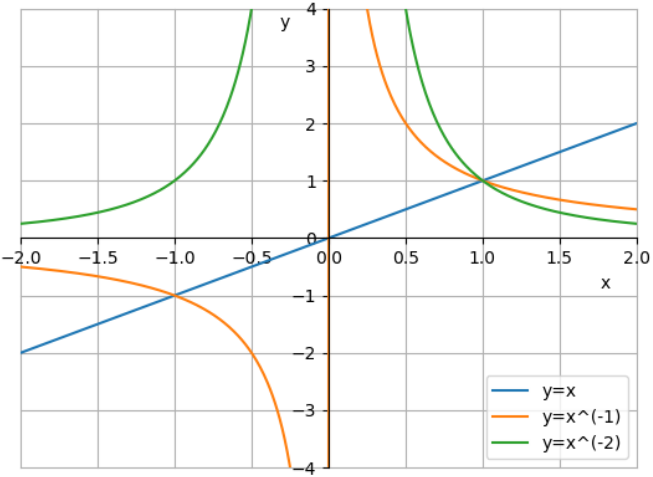
\includegraphics[width=.9\linewidth]{gfx/3/potenze.png}}
\caption{Grafici di funzioni di potenze.}\label{fig:potenze}
\end{figure}

\section{Esponenziale}
Fissata la base $a>0$ con $a \neq 1$, la funzione esponenziale è
\[f(x)=a^x \qquad \dom f = \R \qquad \im f = (0,+\infty)\]
Se si sceglie come base il numero di Nepero $e=2.71828\dots > 1$, la funzione esponenziale si denota:
\[f(x)=e^x=\exp x\]

\subsection{Proprietà}
\begin{enumerate}
	\item se $a>1$, allora la funzzione $a^x$ è strettamente crescente
	\item se $0<a<1$, allora la funzione $a^x$ è strettamente decrescente
	\item se $0<a<b$ con $a,b \neq 1$
	\[\begin{cases}
		a^x<b^x \qquad x>0 \\
		a^x > b^x \qquad x<0
	\end{cases}\]
	\item valgono le seguenti proprietà:
	\begin{itemize}
	\item $a^0=1$
	\item $a^1=a$
	\item $a^{x_1+x_2}=a^{x_1+x_2} \qquad x_1,x_2 \in \R$
	\item $a^{-x}=(\frac{1}{a})^x \qquad x \in \R$
	\item $(a^x)^b = a^{bx} \qquad x,b \in \R$
	\end{itemize}
\end{enumerate}

\begin{figure}[H]
{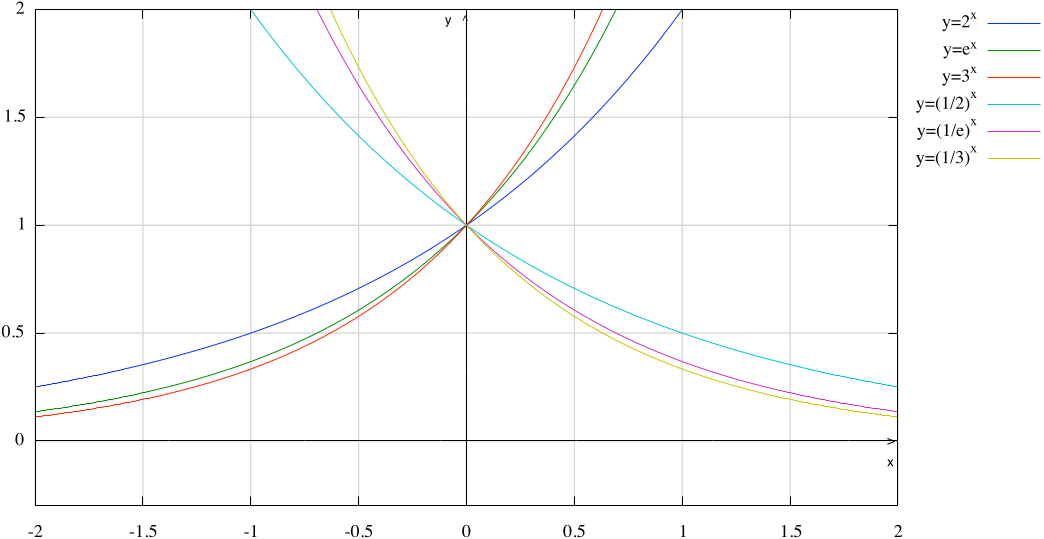
\includegraphics[width=.9\linewidth]{gfx/3/esponenziali.png}}
\caption{Grafici di funzioni esponenziali.}\label{fig:esponenziali}
\end{figure}

\section{Logaritmo}
Fissata la base $a>0$ con $a\neq 1$, la funzione logaritmo
\[f(x)=\log_a x \qquad \dom f = (0,+\infty) \qquad \im f = \R\]
è definita come la funzione inversa della funzione esponenziale $a^x$. Se si sceglie come base il numero di Nepero \textit{e}, il logaritmo si denota:
\[f(x)=\log_e = \log x = \ln x\]

\begin{enumerate}
	\item se $a>1$, allora la funzione $\log_a x$ è strettamente crescente
	\item se $0<a<1$, allora la funzione $\log_a x$ è strettamente decrescente
	\item se $0<a<b$ con $a,b\neq 1$
	\[\begin{cases}
	\log_a x > \log_b x \qquad se x>1 \\
	\log_a x < \log_b x \qquad se 0<x<1 \\
	\end{cases}\]
	\item valgono le seguenti proprietà:
	\begin{itemize}
		\item $\log_a a^x = x \qquad x>1$
		\item $a^{\log_a x}=x \qquad x>0$
		\item $\log_a 1 = 0$
		\item $\log_a a = 1$
		\item $\log_a (x_1 x_2)= \log_a x_1 + \log_a x_2 \qquad x_1,x_2 > 0$
		\item $\log_a (\frac{x_1}{x_2})=\log_a x_1 - \log_a x_2 \qquad x_1,x_2 > 0$
		\item $\log_a x^b = b \log_a x \qquad x>0, b \in \R$
		\item $\log_a x= \frac{\log_b x}{\log_b a}=\frac{\ln x}{\ln a}\qquad x>0,b>0,b\neq 1$
		\item $a^x = e^{(\ln a)x} \qquad x\in \R, a>0, a \neq 1$
	\end{itemize}
\end{enumerate}

\begin{figure}[H]
{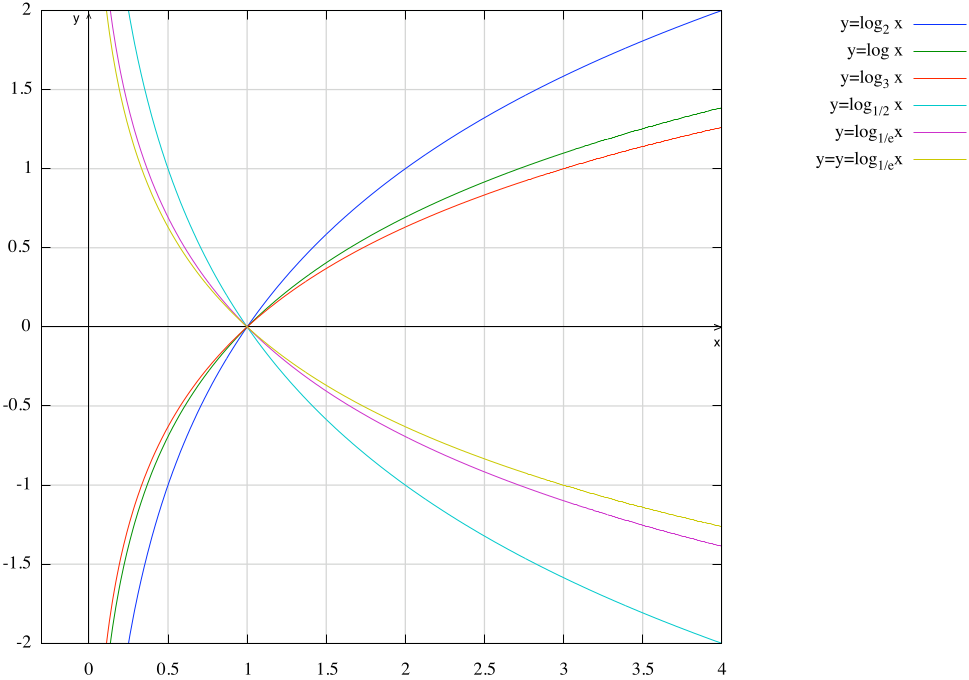
\includegraphics[width=.9\linewidth]{gfx/3/logaritmi.png}}
\caption{Grafici di funzioni logaritmiche.}\label{fig:logaritmi}
\end{figure}
% Chapter X

\chapter{Funzioni trigonometriche} % Chapter title

\label{ch:trigonometria} % For referencing the chapter elsewhere, use \autoref{ch:name}

\section{Radianti}

Sia $\gamma$ una circonferenza di raggio $1$ (detta circonferenza goniometrica) il cui centro $O$ è anche l'origine di un sistema di assi cartesiani e sia $A$ il punto $(1,0)$.
Partendo da $A$ percorriamo la circonferenza in senso antiorario oppure in senso orario.
Sia $x$ un numero reale, denotiamo con $P_x$ il punto su $\gamma$ che si ottiene percorrendo la circonferenza a partire dal punto $A$ per un arco di lunghezza $|x|$, in senso antorario se $x \geq 0$, oppure in senso orario se $x<0$.
Il punto $P_x$ individua un angolo nel piano avente vertice $O$ e delimitatio dalle semirette nel piano uscenti da $O$ e passanti per $A$ e per $P_x$.
Il numero reale $x$ rappresenta la misura dell'angolo in radianti.

\begin{wrapfigure}{r}{0.45\textwidth}
  \begin{center}
    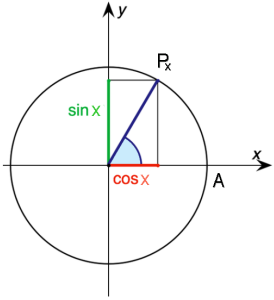
\includegraphics[width=0.42\textwidth]{gfx/4/circonferenza.png}
  \end{center}
  \caption{Circonferenza goniometrica}\label{fig:goniometrica}
\end{wrapfigure}

La relazione tra radianti e gradi è data da:
\[\frac{\gamma_{\text{radianti}}}{2\pi}=\frac{\gamma_{\text{gradi}}}{360}\]

Osserviamo che l'incremento della lunghezza $x$ di $2\pi$ corrisponde a compiere un intero giro sulla circonferenza in senso antiorario ritornando al punto $P_x$ (così come decrementare di $2\pi$ la lunghezza $x$). Quindi si ha:
\[P_{x\pm k2\pi}=P_x \qquad \forall x \in \R, k \in \N\]

\section{Le funzioni seno e coseno}
Una funzione $f:\R \in \R$ è detta periodica di periodo $T$, $T>0$ se:
\[f(x+T)=f(x) \forall x \in \R\]
La caratteristica fondamentale delle funzioni periodiche è che i suoi valori si ripetono dopo intervalli di ampiezza $T$.

\subsection{Simmetria}
Indichiamo con $\cos x$ e con $\sin x$ rispettivamente l'ascissa e l'ordinata del punto $P_x$. Le funzioni $y=\cos x$ e $y=\sin x$ sono definite su $\R$ a valori nell'intervallo $[-1,1]$, sono periodiche di minimo periodo $2\pi$ e soddisfano la relazione:
\[\sin^2 x + \cos^2 x = 1\]

\subsection{Monotonia} Per la periodicità di seno e coseno ci basta studiarne le proprietà nell'intervallo $[0,2\pi]$. Dalle definizioni segue subito che la funzione seno è dispari e la funzione coseno è pari; inoltre la funzione coseno è strettamente decrescente in $[0,\pi]$ e strettamente crescente in $[\pi,2\pi]$. La funzione seno è strettamente crescente in $[0,\frac{\pi}{2}] \cup [\frac{3}{2}\pi,2\pi)$ e strettamente decrescente in $[\frac{\pi}{2},\frac{3}{2}\pi]$.

\begin{figure}[H]
{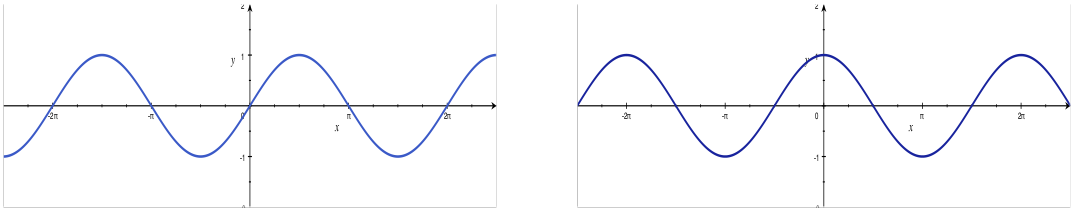
\includegraphics[width=1\linewidth]{gfx/4/senocoseno.png}}
\caption{Grafico delle funzioni: seno e coseno}\label{fig:seno-coseno}
\end{figure}

\subsection{Formule trigonometriche}
\subsubsection{Formule di addizione e sottrazione}
\[\sin(\alpha\pm\beta)=\sin(\alpha)\cos(\beta)\pm\cos(\alpha)\sin(\beta)\]
\[\cos(\alpha\pm\beta)=\cos(\alpha)\cos(\beta)\mp\sin(\alpha)\sin(\beta)\]
\subsubsection{Formule di duplicazione}
\[\sin(2x)=2\sin x\cos x\]
\[\cos(2x)=2\cos^2 x - 1\]
\subsubsection{Formule di potenza}
\[(\sin x)^2 = \sin^2 x= \frac{1-\cos(2x)}{2}\]
\[(\cos x)^2 = \cos^2 x= \frac{1+\cos(2x)}{2}\]
\subsubsection{Formule di bisezione}
\[\sin(\frac{x}{2})=\sqrt{\frac{1-\cos x}{2}} \qquad 0<x\leq 2\pi\]
\[\cos(\frac{x}{2})=\sqrt{\frac{1+\cos x}{2}} \qquad -\pi<x\leq \pi\]
\subsubsection{Formule di prostaferesi}
\[\sin x -\sin y=2\sin(\frac{x-y}{2})\cos(\frac{x+y}{2})\]
\[\cos x -\cos y=-2\cos(\frac{x-y}{2})\sin(\frac{x+y}{2})\]


\[\cos(x+\pi)=-\cos x \qquad \sin(x+\pi)=-\sin x\]
\[\cos(x+\frac{\pi}{2})=-\sin x \qquad \sin(x+\frac{\pi}{2})=\cos x \]

\section{La funzione tangente}
\begin{wrapfigure}{r}{0.45\textwidth}
  \begin{center}
    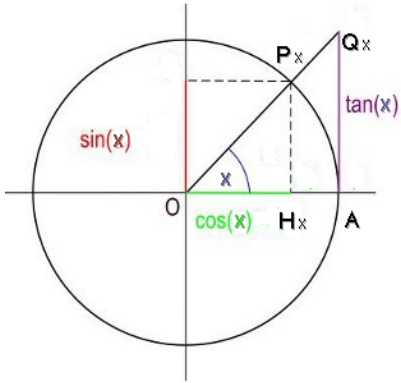
\includegraphics[width=0.42\textwidth]{gfx/4/tangente.png}
  \end{center}
  \caption{Tangente.}\label{fig:circo-tangente}
\end{wrapfigure}

La funzione tangente è:
\[\tan x = \frac{\sin x}{\cos x}\]
Definita nei punti di $\R$ diversi da $\frac{\pi}{2} +k\pi,k\in\Z$ e, come vedremo in seguito, ha immagine $\R$.
La funzione tangente è periodica per: $(x)=\tan(x+k\pi)$ per $k\in \Z$ cioè $\tan(x)$ è periodica di minimo periodo $T=\pi$.

Nella \autoref{fig:circo-tangente} è evidenziata la tangente nel punto $(A,Q_x=\tan(x))$.

\subsection{Simmetria}
Dalle proprietà di simmetria delle funzioni seno e coseno, si deduce che la funzione tangente è dispari: il rapporto di una funzione pari e di una funzione dispari è dispari.

\subsection{Monotonia}
La funzione tangente è strettamente crescente in ogni intervallo $(\frac{-\pi}{2}+k\pi,\frac{\pi}{2}+k\pi), k\in \Z$

\begin{figure}[H]
{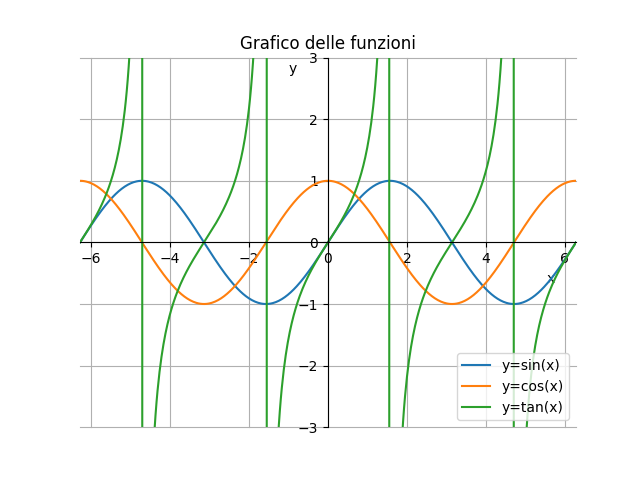
\includegraphics[width=.9\linewidth]{gfx/4/trigonometriche.png}}
\caption{Funzioni trigonometriche}\label{fig:trigonometriche}
\end{figure}

\section{Funzioni trigonometriche inverse}
Le funzioni trigonometriche inverse sono definite come, il dominio della funzione di partenza è stato ristretto per permettere l'inversione della funzione.

\[\arcsin x = f^{-1}(x) \qquad f(x)=\sin(x) \qquad x\in [\frac{-\pi}{2}, \frac{\pi}{2}]\]
\[\arccos x = f^{-1}(x) \qquad f(x)=\cos(x) \qquad x\in [0, \pi]\]
\[\arctan x = f^{-1}(x) \qquad f(x)=\tan(x) \qquad x\in (\frac{-\pi}{2}, \frac{\pi}{2})\]

\subsection{Dominio ed immagine}
\[\dom \arcsin x = [-1,1] \qquad \dom \arccos x = [-1,1] \qquad \dom \arctan x = \R\]
\[\im \arcsin x = [\frac{-\pi}{2}, \frac{\pi}{2}] \qquad \im \arccos x = [0, \pi], \qquad \im \arctan x = (\frac{-\pi}{2}, \frac{\pi}{2})\]

\subsection{Parità}
\[\arcsin(-x)=-\arcsin x\]
\[\arctan(-x)=-\arctan x\]

\subsection{Monotonia}
\begin{itemize}
\item la funzione $\arcsin x$ è strettamente crescente
\item la funzione $\arccos x$ è strettamente decrescente
\item la funzione $\arctan x$ è strettamente crescente
\end{itemize}

\subsection{Relazioni}
\[\arcsin x + \arccos x = \frac{\pi}{2}\]
\[\arccos(-x) = \pi - \arccos(x)\]
\[\arctan x + \arctan (\frac{1}{x}) = \begin{cases}
 \frac{\pi}{2} \quad x>0 \\
 \frac{-\pi}{2} \quad x<0
\end{cases}\]

\begin{figure}[H]
{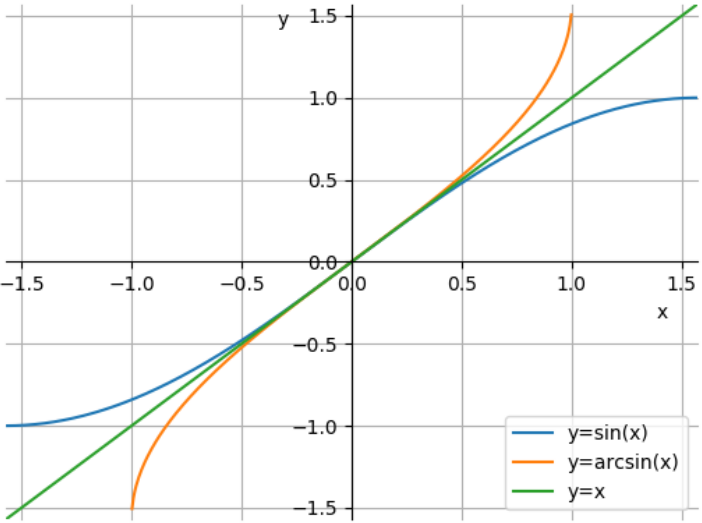
\includegraphics[width=.90\linewidth]{gfx/4/arcoseno.png}}
\caption{Arcoseno.}\label{fig:arcoseno}
\end{figure}

\begin{figure}[H]
{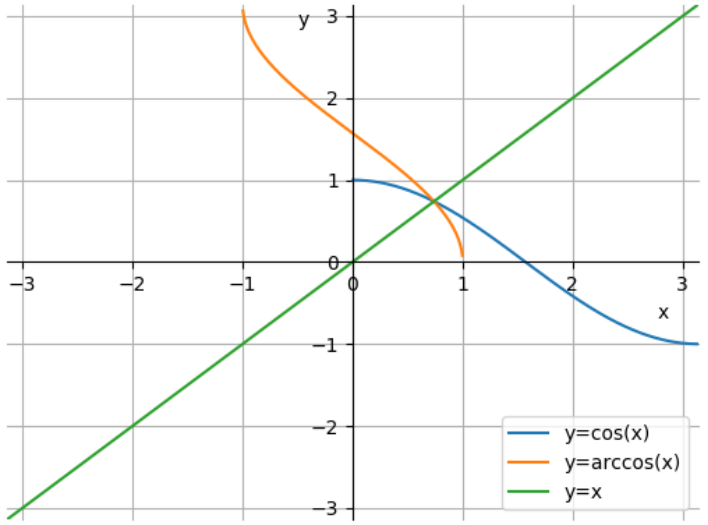
\includegraphics[width=.90\linewidth]{gfx/4/arcocoseno.png}
}
\caption{Arcocoseno.}\label{fig:arcocoseno}
\end{figure}

\begin{figure}[H]
{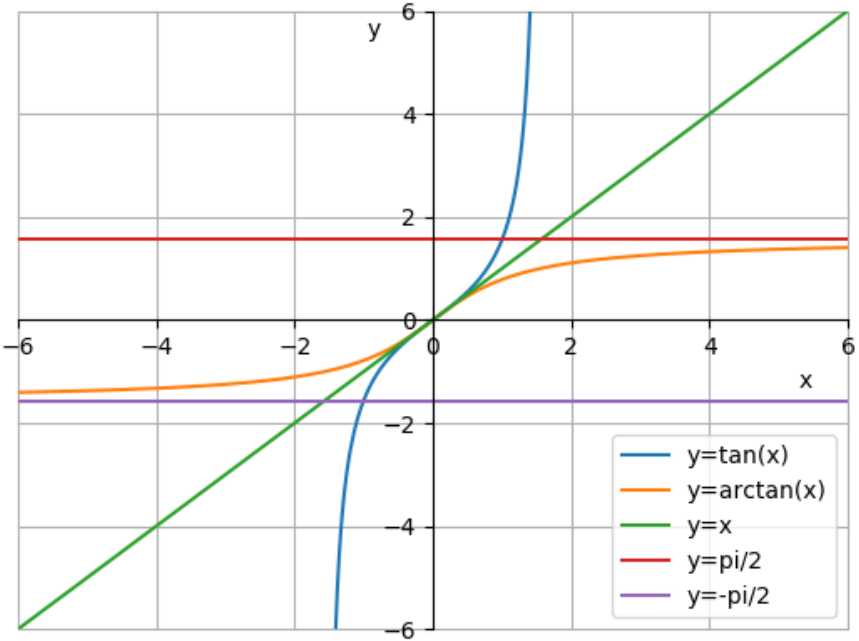
\includegraphics[width=.90\linewidth]{gfx/4/arcotangente.png}}
\caption{Arcotangente.}\label{fig:arcotangente}
\end{figure}


\cleardoublepage
%\ctparttext{}
\part{Funzioni continue e limiti}\label{pt:limiti}
% Chapter X

\chapter{Funzioni continue} % Chapter title

\label{ch:continue} % For referencing the chapter elsewhere, use \autoref{ch:name}

%----------------------------------------------------------------------------------------

\section{Funzioni continue}

Data una funzione $f:A\rightarrow \R, y = f(x)$, ed un punto $x_0 \in A $, la funzione è detta continua in $x_0$ se per ogni $\epsilon > 0$ esiste $\delta > 0$ tale che:
\[f(x_0)-\epsilon < f(x) < f(x_0) + \epsilon \qquad \forall x \in A \cap x_0 - \delta < x < x_0 + \delta \]

La funzione è detta continua se è continua in $x_0$ per ogni $x_0 \in A$.

\begin{teo}[Continuità funzioni elementari]
Le funzioni potenza $x^a$, esponenziali $a^x$, logaritmo $\log_a x$, trigonometriche e trigonometriche inverse, sono continue.
\end{teo}

\begin{teo}[Algebra delle funzioni continue]
Date due funzioni $f,g: A \rightarrow \R, \quad y=f(x), \quad y=g(x)$, continue, allora:
\begin{enumerate}
\item la somma $f(x) + g(x)$ è una funzione continua;
\item il prodotto $f(x)g(x)$ è una funzione continua;
\item il rapporto $\frac{f(x)}{g(x)}$ è una funzione continua sul suo dominio ${x\in A | g(x) \neq 0 }$
\end{enumerate}
\end{teo}

\begin{teo}[Continuità funzione composta]
Date due funzioni continue $f:A\rightarrow \R$ e $g:B\rightarrow \R$ allora la funzione composta:
\[g\circ f:{x\in A |f(x) \in B} \rightarrow \R \qquad y=g(f(x))\]
è continua.
\end{teo}

\begin{teo}[Continuità funzioni inversa]
Data una funzione $f:I\rightarrow \R, \quad y=f(x)$, tale che:
\begin{enumerate}
\item $f$ è iniettiva;
\item $f$ è continua;
\item il dominio di $I$ è un intervallo;
\end{enumerate}
allora, posto $B = \im f$, la funzione inversa $f^{-1}:B\rightarrow \R$ è continua.
\end{teo}

% Chapter 6

\chapter{Limiti} % Chapter title

\label{ch:limiti} % For referencing the chapter elsewhere, use \autoref{ch:name}

%----------------------------------------------------------------------------------------

\section{Punto di accumulazione}
Dato un insieme $A \subseteq \R$ e:
\begin{enumerate}
\item un punto $x_0 \in \R$ è detto punto di accumulazione per $A$ se per ogni $\delta > 0$ esiste $x\in A$ tale che:
\[x_0-\delta <x<x_0+\delta \qquad x \neq x_0\]
\item $+\infty$ è detto punto di accumulazione per $A$ se per ogni $R>0$ esiste $x\in A$ tale che $x>R$
\item $-\infty$ è detto punto di accumulazione per $A$ se per ogni $R>0$ esiste $x\in A$ tale che $x<-R$
\end{enumerate}

\section{Limite}
Data una funzione $f:A\rightarrow \R$, un punto di accumulazione $x_0\in\R\cup\{\pm\infty\}$ per $A$ ed $\ell\in\R\cup\{\pm\infty\}$, si scrive
\[\lim_{x\to x_0}{f(x)=\ell}\]
Si distinguono i casi:
\begin{enumerate}
\item $x_0\in \R$ e $\ell \in \R$: se per ogni $\epsilon > 0$ esiste $\delta > 0$ tale che:
\[\ell - \epsilon < f(x) < \ell + \epsilon \qquad \forall x\in A,x\neq x_0 \cap x_0 - \delta < x < x_0 + \delta\]

\item $x_0\in \R$ e $\ell = \pm \infty$: se per ogni $M > 0$ esiste $\delta > 0$ tale che:
\[\begin{cases}
f(x)>M & \text{se } \ell=+\infty \\
f(x)<-M & \text{se } \ell=-\infty
\end{cases}
\quad
\forall x\in A, x\neq x_0 \cap x_0 - \delta < x < x_0 + \delta
\]

\item $x_0 = \pm \infty$ e $\ell = \in \R$: se per ogni $\epsilon > 0$ esiste $R > 0$ tale che:
\[\ell-\epsilon<f(x)<\ell+\epsilon \quad \forall x\in A \cap
\begin{cases}
x>R & \text{se } x_0=+\infty \\
x<-R & \text{se } x_0=-\infty
\end{cases}\]

\item $x_0 = \pm \infty$ e $\ell = \in \R$: se per ogni $M > 0$ esiste $R > 0$ tale che:
\[\begin{cases}
f(x)>M & \text{se } \ell=+\infty \\
f(x)<-M & \text{se } \ell=-\infty 
\end{cases}
\quad \forall x\in A \cap
\begin{cases}
x>R & \text{se } x_0=+\infty \\
x<-R & \text{se } x_0=-\infty
\end{cases}
\]
\end{enumerate}

In tal caso, si dice che esiste finito il limite di $f$ per $x$ che tende a $x_0$ e vale $\ell$ oppure che $f(x)$ tende ad $\ell$ per $x$ che tende a $x_0$.

\begin{prop}[Continuità dei limiti]
Data $f:A\rightarrow \R$ ed $x_0\in A$ punto di accumulazione per $A$, $f$ è continua in $x_0$ se e solo se:
\[\lim_{x\to x_0}{f(x)}=f(x_0)\]
\end{prop}

\subsection{Limite destro e sinitro}
Data una funzione $f:A\rightarrow \R$ ed un punto $x_0 \in \R$ per $A$ tale che per ogni $\delta>0$
\[A\cap (-\delta,x_0)\neq \emptyset \qquad \text{e} \qquad A\cap (x_0,\delta)\neq \emptyset\]
si scrive:
\[\begin{cases}
\lim_{x\to x_{0^+}}{f(x)}=\ell_1 \in \R & \text{limite destro} \\
\lim_{x\to x_{0^-}}{f(x)}=\ell_2 \in \R & \text{limite sinistro}
\end{cases}\]
Se per ogni $\epsilon >0$ esiste $\delta > 0$ tale che:
\[\begin{cases}
\ell_1 - \epsilon < f(x) < \ell_1 + \epsilon \\
\ell_2 - \epsilon < f(x) < \ell_2 + \epsilon \\
\end{cases}
\qquad \forall x\in A \cap
\begin{cases}
x_0<x<x_0+\delta & \text{limite destro}\\
x_0-\delta<x<x_0 & \text{limite sinistro}\\
\end{cases}\]
Analoghe definizioni valgono se $\ell_{1,2}=\pm\infty$

\begin{prop}
Data una funzione $f:A\rightarrow \R$, un punto $x_0\in \R$ tale che per ogni $\delta>0$
\[A\cap(-\delta,x_0) \neq \emptyset \qquad \text{e} \qquad A\cap(x_0,\delta) \neq \emptyset)\]
Allora $x_0$ è un punto di accumulazione per $A$ e:
\[\text{esiste } \lim_{x\to x_0}f(x)=\ell \quad \Leftrightarrow \quad \text{esistono }
\begin{cases}
\lim_{x\to x_{0^+}}{f(x)}=\ell \\
\lim_{x\to x_{0^-}}{f(x)}=\ell
\end{cases}\]
\end{prop}

\begin{teo}[Algebra dei limiti]
Date due funzioni $f,g:A\rightarrow\R$ ed un punto $x_0\in\R$ di accumulazione per $A$, se esitono:
\[\lim_{x\to x_0}{f(x)}=\ell_1\in\R\cup\{\pm\infty\}\]
\[\lim_{x\to x_0}{f(x)}=\ell_2\in\R\cup\{\pm\infty\}\]
allora:
\begin{description}
\item[Somma:]
\[\lim_{x\to x_0}{f(x)+g(x)}= 
\begin{array}{ |*{4}{c|} }
\toprule
& \ell_2 \in \R & \ell_2 = +\infty & \ell_2 = -\infty \\
\midrule
\ell_1 \in \R & \ell_1 + \ell_2 & +\infty & -\infty \\
\midrule
\ell_1 = +\infty & +\infty & +\infty & \foi \\
\midrule
\ell_1 = -\infty & -\infty & \foi & -\infty \\
\bottomrule
\end{array}\]
Dove $\foi$= forma indeterminata $+\infty -\infty$

\item[Prodotto:]
\[\lim_{x\to x_0}{f(x)g(x)}= 
\begin{array}{ |*{6}{c|} }
\toprule
& \ell_2<0 & \ell_2=0 & \ell_2>0 & \ell_2=+\infty & \ell_2=-\infty\\
\midrule
\ell_1<0 & \ell_1 \ell_2 & 0 & \ell_1 \ell_2 & -\infty & +\infty \\
\midrule
\ell_1=0 & 0 & 0 & 0 & \foi & \foi \\
\midrule
\ell_1>0 & \ell_1 \ell_2 & 0 & \ell_1 \ell_2 & +\infty & -\infty \\
\midrule
\ell_1=+\infty & -\infty & \foi & +\infty & +\infty & -\infty \\
\midrule
\ell_1=-\infty & +\infty & \foi & -\infty & -\infty & +\infty\\
\bottomrule
\end{array}\]
Dove $\foi$= forma indeterminata $0 \infty$

\item[Rapporto:]
\[\lim_{x\to x_0}{\frac{f(x)}{g(x)}}=
\begin{array}{ |*{6}{c|} }
\toprule
& \ell_2<0 & \ell_2=0^{\pm} & \ell_2>0 & \ell_2=+\infty & \ell_2=-\infty\\
\midrule
\ell_1<0 & \frac{\ell_1}{\ell_2} & \mp\infty & \frac{\ell_1}{\ell_2} & 0 & 0 \\
\midrule
\ell_1=0 & 0 & \foi & 0 & 0 & 0 \\
\midrule
\ell_1>0 & \frac{\ell_1}{\ell_2} & \pm\infty & \frac{\ell_1}{\ell_2} & 0 & 0 \\
\midrule
\ell_1=+\infty & -\infty & \pm\infty & +\infty & \foi & \foi \\
\midrule
\ell_1=-\infty & +\infty & \mp\infty & -\infty & \foi & \foi \\
\bottomrule
\end{array}
\]
Dove $\foi$= forma indeterminata $\frac{0}{0}$ o $\frac{\infty}{\infty}$ e la notazione $l_2=0^\pm$ significa che:
\begin{enumerate}
\item esiste il limite
\[\lim_{x\to x_0}{g(x)}=0\]
\item esiste $\delta>0$ tale che per ogni $x\in A \cap (x_0-\delta,x_0+\delta), x\neq x_0$
\[\begin{cases}
g(x)>0 & \ell_2 = 0^+ \\
g(x)<0 & \ell_2 = 0^- \\
\end{cases}\]
Se $x_0 \in \R$ (analoga definizione se $x_0=\pm\infty$).
\end{enumerate}
\end{description}
\end{teo}

\begin{teo}[Limite funzione composta.]
Date due funzioni $f:A\rightarrow\R,y=f(x)$ e $g:B\rightarrow\R,z=g(y)$, tali che:
\begin{enumerate}
\item per ogni $x\in A$, allora $f(x)\in B,$
\item il punto $x_0$ è di accumulazione per $A$ ed esiste:
\[\lim_{x\to x_0}{f(x)}=y_0\in\R\cup\{+\infty\},\]
\item il punto $y_0$ è di accumulazione per $B$ ed esiste:
\[\lim_{y\to y_0}{g(x)}=\ell\in\R\cup\{+\infty\},\]
\end{enumerate}
Allora esiste:
\[\lim_{x\to x_0}{g(f(x))}=\ell\]
\paragraph{Nota:}
Le condizioni del teorema non sono sufficienti per assicurare l'esistenza del limite $\lim_{x\to x_0}{g(f(x))}=\ell$. Occorre aggiungere delle ipotesi tecniche, che però sono sempre verificate negli esercizi. Ad esempio, è sufficiente richiedere che una delle seguenti tre condizioni sia soddisfatta:
\begin{enumerate}
\item il punto $y_0$ non appartiene a $\dom{g}$;
\item la funzione $g$ è continua in $y_0$;
\item esiste $\delta>0$ tale che $f(x)\neq y_0$ per ogni $x\in A,x\neq x_0$ e $x_0-\delta\leq x\leq x_0+\delta$.
\end{enumerate}
\end{teo}

\part{Derivate}
% Chapter 6

%\chapter{Intorno} % Chapter title

%\label{ch:intorno} % For referencing the chapter elsewhere, use \autoref{ch:name}

%----------------------------------------------------------------------------------------


%\include{multiToC} % <--- just debug stuff, ignore for your documents
% ********************************************************************
% Backmatter
%*******************************************************
%\appendix
%\renewcommand{\thechapter}{\alph{chapter}}
%\cleardoublepage
%\part{Appendix}
%% Chapter 0a

\chapter{Studio di funzioni} % Chapter title

\label{ch:studio-di-funzioni} % For referencing the chapter elsewhere, use \autoref{ch:name}

%----------------------------------------------------------------------------------------
Lo schema seguente indica i passi principali da seguire per svolgere lo studio di funzioni.

Ogni volta che si è risolto un punto occorre rappresentare l'informazione sul grafico e verificare che sia in accordo con quanto dedotto precedentemente.

\begin{enumerate}
\item Determinare il dominio della funzione $f$ e scriverlo come unione di intervalli:
\[\dom f = I_0 \cup I_1 \cup \dots \]

\item Studiare il segno della funzione e calcolare le intersezioni con gli assi cartesiani: $f(0)$ se $0\in\dom f$ e risolvere l'equazione $f(x)=0$.

\item Stabilire se la funzione è continua, quante vole è derivabile e calcolare $f^\prime$ ed $f^{\prime\prime}$.

\item Calcolare i limiti di $f$ agli estremi di ciascun intervallo, $I_1, I_2 \dots$

\item Studiare il segno della derivata prima $f^\prime$ calcolando i punti critici, deducendo gli intervalli di monotonia della funzione (teorema della caratterizzazione della monotonia).

\item Determinare i punti di massimo e minimo relativi, ricordando che il teorema della condizione necessaria del I ordine dà solo una condizione necessaria affinchè un punto sua un estremo relativo.
\begin{aenumerate}
\item I punti critici $x_0$ (non coincidenti con gli estremi degli intervalli $I_1, I_2 \dots$) in cui la derivata \textit{cambia segno} sono punti di estremo relativo. Infatti, se:
\[\begin{cases}
f^\prime(x)<0 \text{    se } x_0< \delta < x < x_0 \\
f^\prime(x)>0 \text{    se } x_0< \delta < x < x_0 \\
\end{cases}\]
allota $x_0$ è un punto di minimo relativo.
Analogamente se:
\[\begin{cases}
f^\prime(x)>0 \text{    se } x_0< \delta < x < x_0 \\
f^\prime(x)<0 \text{    se } x_0< \delta < x < x_0 \\
\end{cases}\]
allora $x_0$ è un punto di massimo relativo.
Per tali valori, calcolare il corrispondente estremo relativo $f(x_0)$.

\item Verificare se gli estremi degli intervalli $I_1, I_2 \dots$, purchè appartenenti al dominio, siano punti di estremi relativi (in tali punti in generale la derivata prima non si annulla).
Ad esempio se $I_1=[a,b)$ e:
\[f^\prime(x)>0 \qquad a<x<a+\delta\]
allora $x_0=a$ è un punto di minimo relativo, mentre $b\not\in\dom f$ per cui non ha senso chiedersi se sia un punto di estremo relativo.

\item Se lo studio del segno di $f^\prime$ non si può svolgere, ma si riesce a calcolare i punti critici $f^\prime(x_0)=0$, allora il segno di $f^{\prime\prime}(x_0)$ permette di stabilire se è un punto di estremo relativo (Corollario della condizione sufficiente del secondo ordine per estremi relativi).
\end{aenumerate}

\item Determinare $\inf f$ e $\sup f$, stabilendo se sono o meno minimo e massimo assoluti.

\item Determinare l'immagine di $f$ utilizzando il teorema dei valori intermedi.

\item Studiare il segno della derivata seconda $f^{\prime\prime}$ e dedurne gli intervalli di convessità e concavità della funzione (teorema della caratterizzazione convessità).
In particolare i punti in cui $f^{\prime\prime}$ cambia segno, son odetti punti di flesso e, in tali punti, può essere utile calcolare la derivata e tracciare la retta tangente.
\end{enumerate}

In molti casi non si riescono a svolgere esplicitamente i calcoli per tutti i punti e si dovrà dedurre l'andamento del grafico solo attraverso i punti svolti.
%********************************************************************
% Other Stuff in the Back
%*******************************************************
%\cleardoublepage%********************************************************************
% Bibliography
%*******************************************************
% work-around to have small caps also here in the headline
% https://tex.stackexchange.com/questions/188126/wrong-header-in-bibliography-classicthesis
% Thanks to Enrico Gregorio
\defbibheading{bibintoc}[\bibname]{%
  \phantomsection
  \manualmark
  \markboth{\spacedlowsmallcaps{#1}}{\spacedlowsmallcaps{#1}}%
  \addtocontents{toc}{\protect\vspace{\beforebibskip}}%
  \addcontentsline{toc}{chapter}{\tocEntry{#1}}%
  \chapter*{#1}%
}
\printbibliography[heading=bibintoc]

% Old version, will be removed later
% work-around to have small caps also here in the headline
%\manualmark
%\markboth{\spacedlowsmallcaps{\bibname}}{\spacedlowsmallcaps{\bibname}} % work-around to have small caps also
%\phantomsection
%\refstepcounter{dummy}
%\addtocontents{toc}{\protect\vspace{\beforebibskip}} % to have the bib a bit from the rest in the toc
%\addcontentsline{toc}{chapter}{\tocEntry{\bibname}}
%\label{app:bibliography}
%\printbibliography

%\cleardoublepage%*******************************************************
% Declaration
%*******************************************************
\pdfbookmark[0]{Declaration}{declaration}
\chapter*{Declaration}
\thispagestyle{empty}
Put your declaration here.
\bigskip

\noindent\textit{\myLocation, \myTime}

\smallskip

\begin{flushright}
    \begin{tabular}{m{5cm}}
        \\ \hline
        \centering\myName \\
    \end{tabular}
\end{flushright}

%\cleardoublepage\pagestyle{empty}

\hfill

\vfill


\pdfbookmark[0]{Colophon}{colophon}
\section*{Colophon}
This document was typeset using the typographical look-and-feel \texttt{classicthesis} developed by Andr\'e Miede and Ivo Pletikosić.
The style was inspired by Robert Bringhurst's seminal book on typography ``\emph{The Elements of Typographic Style}''.
\texttt{classicthesis} is available for both \LaTeX\ and \mLyX:
\begin{center}
\url{https://bitbucket.org/amiede/classicthesis/}
\end{center}
Happy users of \texttt{classicthesis} usually send a real postcard to the author, a collection of postcards received so far is featured here:
\begin{center}
\url{http://postcards.miede.de/}
\end{center}
Thank you very much for your feedback and contribution.

\bigskip

\noindent\finalVersionString

%Hermann Zapf's \emph{Palatino} and \emph{Euler} type faces (Type~1 PostScript fonts \emph{URW
%Palladio L} and \emph{FPL}) are used. The ``typewriter'' text is typeset in \emph{Bera Mono},
%originally developed by Bitstream, Inc. as ``Bitstream Vera''. (Type~1 PostScript fonts were made
%available by Malte Rosenau and
%Ulrich Dirr.)

%\paragraph{note:} The custom size of the textblock was calculated
%using the directions given by Mr. Bringhurst (pages 26--29 and
%175/176). 10~pt Palatino needs  133.21~pt for the string
%``abcdefghijklmnopqrstuvwxyz''. This yields a good line length between
%24--26~pc (288--312~pt). Using a ``\emph{double square textblock}''
%with a 1:2 ratio this results in a textblock of 312:624~pt (which
%includes the headline in this design). A good alternative would be the
%``\emph{golden section textblock}'' with a ratio of 1:1.62, here
%312:505.44~pt. For comparison, \texttt{DIV9} of the \texttt{typearea}
%package results in a line length of 389~pt (32.4~pc), which is by far
%too long. However, this information will only be of interest for
%hardcore pseudo-typographers like me.%
%
%To make your own calculations, use the following commands and look up
%the corresponding lengths in the book:
%\begin{verbatim}
%    \settowidth{\abcd}{abcdefghijklmnopqrstuvwxyz}
%    \the\abcd\ % prints the value of the length
%\end{verbatim}
%Please see the file \texttt{classicthesis.sty} for some precalculated
%values for Palatino and Minion.
%
%    \settowidth{\abcd}{abcdefghijklmnopqrstuvwxyz}
%    \the\abcd\ % prints the value of the length

% ********************************************************************
% Game Over: Restore, Restart, or Quit?
%*******************************************************
\end{document}
% ********************************************************************
